% SPDX-License-Identifier: CC-BY-4.0
% Copyright (c) 2026 Alexander Stephen Donahue (ORCID: 0009-0006-8168-9648)
\documentclass[11pt,reqno]{amsart}

\usepackage[margin=0.95in]{geometry}
\usepackage{amsmath,amssymb,amsthm,mathtools}
\usepackage{booktabs,array,multirow,tabularx}
\usepackage{graphicx}
\usepackage{xcolor}
\usepackage{microtype}
\usepackage{enumitem}
\usepackage[hidelinks]{hyperref}
\emergencystretch=2em

\definecolor{accentblue}{HTML}{004E89}
\definecolor{accentgreen}{HTML}{1B7A43}
\definecolor{accentorange}{HTML}{B45309}
\definecolor{accentpurple}{HTML}{6B21A8}

\hypersetup{
  colorlinks=true,
  linkcolor=accentblue,
  citecolor=accentgreen,
  urlcolor=accentblue,
  pdftitle={Hantzsche-Wendt Group Rings, All-Prime Type-II Fracton Codes, and 3D Non-Hermitian B4 Eigenvalue Monodromy},
  pdfauthor={Alexander Stephen Donahue}
}

\newtheorem{theorem}{Theorem}[section]
\newtheorem{proposition}[theorem]{Proposition}
\newtheorem{lemma}[theorem]{Lemma}
\newtheorem{corollary}[theorem]{Corollary}
\theoremstyle{definition}
\newtheorem{definition}[theorem]{Definition}
\newtheorem{remark}[theorem]{Remark}
\newtheorem{openproblem}[theorem]{Open Problem}

\newcommand{\Z}{\mathbb{Z}}
\newcommand{\Q}{\mathbb{Q}}
\newcommand{\R}{\mathbb{R}}
\newcommand{\C}{\mathbb{C}}
\newcommand{\F}{\mathbb{F}}
\newcommand{\T}{\mathbb{T}}
\newcommand{\A}{\mathcal{A}}
\newcommand{\supp}{\operatorname{supp}}
\newcommand{\Disc}{\operatorname{Disc}}
\newcommand{\GSD}{\operatorname{GSD}}
\newcommand{\tierK}{\textsf{\scriptsize\textcolor{accentgreen}{kernel-checked}}}
\newcommand{\tierE}{\textsf{\scriptsize\textcolor{accentblue}{exact-comp}}}
\newcommand{\tierN}{\textsf{\scriptsize\textcolor{accentorange}{numerical-approx}}}
\newcommand{\tierO}{\textsf{\scriptsize\textcolor{accentpurple}{open-problem}}}

\title[Hantzsche--Wendt Group Rings, All-Prime Fractons, and $B_4$ Amoebae]{%
Hantzsche--Wendt Group Rings,\\
All-Prime Type-II Fracton Codes, and 3D Non-Hermitian $B_4$ Monodromy:\\
A Zero-Mathlib Six-Kernel Formalization}

\author{Alexander Stephen Donahue}
\address{Independent Researcher, Spokane, WA, USA}
\email{0\_0@0thernes.art}
\urladdr{https://orcid.org/0009-0006-8168-9648}

\subjclass[2020]{Primary 16S34, 81P73, 14T90; Secondary 20F36, 37B15, 03B35.}
\keywords{Kaplansky Unit Conjecture, Hantzsche--Wendt group, Promislow group, Gardam unit, Type-II fracton codes, Haah cubic code, non-Hermitian amoeba, Ronkin function, Artin braid group $B_4$, Lean~4}

\begin{document}

\begin{abstract}
We establish an exact algebraic, arithmetic, and topological bridge uniting three previously
disconnected frontiers of non-commutative algebra, quantum error correction, and non-Hermitian
band topology around the torsion-free Hantzsche--Wendt (Promislow) crystallographic group
$P = \langle a,b \mid a^{-1}b^2a = b^{-2},\, b^{-1}a^2b = a^{-2}\rangle$ and its faithful
$4$-band Bloch embedding $\Psi : R[P] \hookrightarrow M_4(R[x^{\pm 1}, y^{\pm 1}, z^{\pm 1}])$.
In \textbf{Pillar~I}, we prove universal Klein four-group $V_4$-invariance of
$\det(\Psi(u)-EI_4)$, deduce that every unit over an integral domain has constant Bloch
determinant, derive exact closed-form determinant factorizations at all $8$ sign points
$s \in \{\pm 1\}^3$, prove that Gardam's $\{0,1\}$-lift $\widetilde{\alpha} \in \Z[P]$ satisfies
the unexpected mod-$4$ congruence $\det\Psi(\widetilde{\alpha}) \equiv 1 \pmod{4}$ across all
$89$ Laurent monomials (yielding a constructive $2$-adic Hensel tower in $(\Z/2^m\Z)[P]^\times$
for all $m \ge 1$), establish a \emph{strengthened $2^{21}$ no-sign-lift obstruction} ruling out
all $\pm 1$ lifts of Gardam's support---even allowing an arbitrary even-sum $p \in \Z[N]$---via
the quaternionic norm barrier $P_1^2 - 31 \notin \{\pm 1\}$, and prove that Gardam's unit induces
a $P$-equivariant, strictly reversible $21$-neighbor linear cellular automaton on $\F_2^P$.
In \textbf{Pillar~II}, we exhaustively classify all $64$ signed Haah cubic codes into four gauge
classes with conic discriminants $\det(2Q) \in \{\pm 4, \pm 8, \pm 12\}$ (smooth for every prime
$p \ge 5$, with exactly $24$ codes degenerating into $\F_9$-conjugate lines at $p=3$), give a
brand-new characteristic-universal proof of the Type-II no-strings property for Haah's Cubic Code~1
across \emph{every} prime $p \ge 2$ and $\operatorname{char} 0$ via six pairwise $\Z[t]$ B\'ezout
identities equal to~$2$, establish an odd-prime torsion floor ruling out $\F_p$-rational odd-order
roots for odd $p \le 19$ with first threshold at $p=23$, $L=11$ ($k_{23}(11)=6$), and construct
the first non-Abelian Hantzsche--Wendt fracton stabilizer codes (both a Gardam-twisted code whose
commutation holds strictly mod~$2$ with a $342$-term integer defect and an intrinsically
non-Abelian code commuting over every commutative ring $R[P]$).
In \textbf{Pillar~III}, we prove a universal $V_4$-convex Ronkin origin-minimum law
$R(0,0,0) \le R(\mu)$ implying exact bipolar skin-effect cancellation
$W_x(k_y,-k_z) = -W_x(k_y,k_z)$, establish an exact quadrilateral characterization of Haah's
$3$D double-amoeba $\A(f)\cap\A(g)$ with algebraic $\mathrm{EP}_2$ Jordan nilpotency, and
demonstrate that fundamental momentum loops of Gardam's $4$-band crystal $\Psi(\widetilde{\alpha})(k)$
generate the entire non-Abelian symmetric group $S_4$ of order $24$ with integer quartic
discriminant braid degrees $\{-1,-2,-3,+3\}$.
All $15$ exact theorems (\textsf{T1a}--\textsf{T3c}) are formalized in zero-Mathlib Lean~4.35.0
with zero \texttt{sorry}, zero \texttt{native\_decide}, and axioms strictly within
$\{\texttt{propext}, \texttt{Classical.choice}, \texttt{Quot.sound}\}$, replayed across six
independent proof kernels and differentially cross-checked against zero-dependency Rust and Python
implementations. Overarching open conjectures (including Kaplansky's Unit Conjecture in
characteristic~$0$) remain explicitly open.
\end{abstract}

\maketitle

\section{Introduction and Scope}
\label{sec:intro}

Three landmark structures in contemporary mathematical physics and algebra share an unexpectedly
rigid geometric backbone, yet have historically been developed in completely separate literatures:
\begin{enumerate}[leftmargin=2em]
  \item \textbf{Non-commutative group rings of crystallographic groups:} Gardam's 2021
    refutation~\cite{gardam2021counterexample} of Kaplansky's Unit Conjecture~\cite{kaplansky1970problems}
    over $\F_2$ (extended to all prime characteristics by Murray~\cite{murray2021more}) lives in the
    group ring of the torsion-free $3$-dimensional Hantzsche--Wendt crystallographic
    group~\cite{hantzsche1935dreidimensionale,promislow1988simple}, also known as the Promislow
    group $P$. Whether $\Q[P]$ or $\Z[P]$ contains nontrivial units---and whether Gottschalk's
    surjunctivity conjecture~\cite{gottschalk1973some,gromov1999endomorphisms} interacts with
    nontrivial group-ring units via reversible cellular automata---remains intensely studied.
  \item \textbf{Type-II fracton quantum stabilizer codes:} Introduced by Chamon~\cite{chamon2005quantum}
    and Haah~\cite{haah2011local,haah2013commuting} and synthesized in the fracton
    literature~\cite{vijay2016fracton,dua2019compactifying,nandkishore2019fractons}, Type-II
    fracton codes are defined by polynomial modules over Abelian translation rings
    $\F_2[x^{\pm 1},y^{\pm 1},z^{\pm 1}]$ whose excitations possess no mobile string logical
    operators. Their arithmetic behavior across odd prime qudit dimensions $p \ge 3$, across all
    $64$ signed variants of Haah's generators, and over genuinely non-Abelian flat $3$-manifold
    group rings $R[P]$ has lacked a unified machine-checked classification.
  \item \textbf{Multi-dimensional non-Hermitian amoebae and multiband braiding:} The amoeba
    formulation of non-Bloch band theory~\cite{passare2004amoebas,wang2024amoeba} expresses the
    non-Hermitian skin effect in arbitrary dimension through the Ronkin potential $R(\mu)$ of a
    Laurent characteristic polynomial, while multiband non-Hermitian Bloch Hamiltonians exhibit
    homotopic eigenvalue braids in Artin's braid group $B_n$ and symmetric monodromy in
    $S_n$~\cite{wojcik2020homotopy,hu2021knots,bergholtz2021exceptional}.
\end{enumerate}

The unifying mechanism of this paper is the faithful $4$-band Bloch representation
$\Psi : R[P] \hookrightarrow M_4(R[x^{\pm 1}, y^{\pm 1}, z^{\pm 1}])$ induced by the index-$4$
normal translation subgroup $N = \langle x, y, z \rangle \cong \Z^3 \trianglelefteq P$ with
point-group quotient $P/N \cong V_4$. Viewed algebraically, $\Psi$ converts Kaplansky unit
obstructions in $\Z[P]$ into $V_4$-symmetric $4 \times 4$ Laurent determinants whose sign-point
specializations factor into quaternionic norms. Viewed quantum-information-theoretically, units
of $\F_2[P]$ conjugate commuting central Haah check operators into genuinely non-Abelian fracton
codes whose CSS commutation can hold strictly mod~$2$ while failing over $\Z[P]$. Viewed
spectrally, any $\{0,1\}$-lift $\widetilde{u} \in \Z[P]$ defines an exact $3$D $4$-band
non-Hermitian Bloch crystal $\Psi(\widetilde{u})(k)$ whose Ronkin potential is forced by
$V_4$-symmetry and convexity to attain its global minimum at $\mu = (0,0,0)$---enforcing exact
bipolar skin cancellation---while its complex eigenvalues braid across $\T^3$ to generate all
$24$ elements of $S_4$.

\subsection{Epistemic Claim Ledger and Verification Boundaries}
\label{sec:claims}

To maintain strict epistemic transparency, Table~\ref{tab:claims} assigns every headline claim in
this manuscript a single verification tier:
\tierK{} (proved in zero-Mathlib Lean~4.35.0 and replayed across six independent kernels),
\tierE{} (verified via exact arbitrary-precision integer/finite-field computation in both Rust
and Python), \tierN{} (floating-point numerical quadrature or complex root tracking with explicit
gap bounds and grid refinement), or \tierO{} (explicitly open conjecture not claimed solved).

\begin{table}[htbp]
\centering
\caption{Numbered claim ledger, Lean~4.35.0 formalization mapping, and epistemic verification tiers.}
\label{tab:claims}
\scriptsize
\setlength{\tabcolsep}{3.5pt}
\begin{tabularx}{\textwidth}{@{}l>{\raggedright\arraybackslash}X>{\raggedright\arraybackslash}p{4.35cm}l@{}}
\toprule
\textbf{ID} & \textbf{Scoped Claim Summary} & \textbf{Lean Declaration / Oracle} & \textbf{Tier} \\
\midrule
\textsf{T1a} & $P$ satisfies Hantzsche--Wendt relations and is torsion-free & \texttt{t1a\_promislow\_group\_}\newline\texttt{torsion\_free} & \tierK{} \\
\textsf{T1b} & $\Psi : R[P] \hookrightarrow M_4(R[N])$ is a faithful homomorphism & \texttt{t1b\_faithful\_four\_band\_}\newline\texttt{bloch\_homomorphism} & \tierK{} \\
\textsf{T1c} & $\det(\Psi(u)-EI_4)$ is $V_4$-invariant; units have constant $\det$ & \texttt{t1c\_universal\_v4\_}\newline\texttt{determinant\_invariance} & \tierK{} \\
\textsf{T1d} & Closed-form factorizations of $\det\Psi(u)$ at all $8$ sign points & \texttt{t1d\_eight\_sign\_point\_}\newline\texttt{factorization} & \tierK{} \\
\textsf{T1e} & Gardam $\alpha\beta=1$ mod~$2$; $89$-term $\det \equiv 1 \pmod 4$; Hensel tower & \texttt{t1e\_gardam\_unit\_mod4\_}\newline\texttt{and\_hensel\_tower} & \tierK{} \\
\textsf{T1f} & Strengthened $2^{21}$ no-sign-lift obstruction ($P_1^2 - 31 \notin \{\pm 1\}$) & \texttt{t1f\_exhaustive\_no\_sign\_}\newline\texttt{lift\_gardam\_support} & \tierK{} \\
\textsf{T1g} & Gardam $21$-neighbor $P$-equivariant reversible linear CA on $\F_2^P$ & \texttt{t1g\_surjunctive\_}\newline\texttt{reversible\_linear\_ca} & \tierK{} \\
\textsf{T2a} & Unit-twisted CSS commutation over arbitrary involutive rings & \texttt{t2a\_nonabelian\_unit\_}\newline\texttt{twisted\_css\_commutation} & \tierK{} \\
\textsf{T2b} & All $64$ signed Haah codes: $\det(2Q) \in \{\pm 4,\pm 8,\pm 12\}$; $p=3$ split & \texttt{t2b\_signed\_haah\_64\_}\newline\texttt{discriminant\_classification} & \tierK{} \\
\textsf{T2c} & Universal all-prime ($p \ge 2$, $\operatorname{char} 0$) Haah CC1 no-strings proof & \texttt{t2c\_universal\_all\_}\newline\texttt{prime\_no\_strings} & \tierK{} \\
\textsf{T2d} & Odd-prime torsion floor ($p \le 19$ empty); first odd-$L$ root $p=23$ & \texttt{t2d\_odd\_prime\_torsion\_}\newline\texttt{and\_p23\_threshold} & \tierK{} \\
\textsf{T2e} & Gardam-twisted ($342$-term $\Z$-defect) \& intrinsic HW fracton codes & \texttt{t2e\_nonabelian\_hw\_}\newline\texttt{fracton\_codes} & \tierK{} \\
\textsf{T3a} & $V_4$-convex Ronkin global minimum strictly at $\mu = (0,0,0)$ & \texttt{t3a\_v4\_convex\_ronkin\_}\newline\texttt{origin\_minimum} & \tierK{} \\
\textsf{T3b} & Haah double-amoeba quadrilateral slice \& algebraic $\mathrm{EP}_2$ ($H^2=0$) & \texttt{t3b\_haah\_amoeba\_}\newline\texttt{and\_ep2\_jordan} & \tierK{} \\
\textsf{T3c} & Artin $B_4$ relations \& full $24$-element $S_4$ closure of Gardam loops & \texttt{t3c\_artin\_b4\_and\_}\newline\texttt{full\_s4\_monodromy} & \tierK{} \\
\midrule
\textsf{E1} & Exact $2$-adic inverse supports ($m=1\dots 6$) \& $k_p(L)$ tables & Rust \texttt{promislow\_core} + Python & \tierE{} \\
\textsf{N1} & Ronkin $R(\mu)$ quadrature, bipolar $W_x$ map, braid degrees & Rust + Python diff ($<10^{-6}$) & \tierN{} \\
\textsf{O1} & Kaplansky Unit Conjecture in $\operatorname{char} 0$, general Gottschalk & Explicitly NOT claimed solved & \tierO{} \\
\bottomrule
\end{tabularx}
\end{table}

\section{Pillar I: Hantzsche--Wendt Group Rings, Mod-4 Collapse, and the Strengthened $2^{21}$ Obstruction}
\label{sec:pillar1}

\subsection{The Promislow Group and Faithful $4$-Band Bloch Embedding}

Let $P = \langle a, b \mid a^{-1} b^2 a = b^{-2},\, b^{-1} a^2 b = a^{-2} \rangle$ be the
Hantzsche--Wendt / Promislow group~\cite{hantzsche1935dreidimensionale,promislow1988simple}.
Setting $x = a^2$, $y = b^2$, and $z = (ab)^2$, the subgroup $N = \langle x, y, z \rangle \cong \Z^3$
is normal of index~$4$ in $P$ with coset representatives $C = \{e, a, b, ab\}$ and quotient
$P/N \cong V_4$. Every element of $P$ has a unique normal form $x^i y^j z^k c$ with
$(i,j,k) \in \Z^3$ and $c \in C$. Conjugation by $c \in C$ acts on $N$ via the $V_4$-sign
characters
\[
  \sigma_e = (+,+,+), \qquad \sigma_a = (+,-,-), \qquad \sigma_b = (-,+,-), \qquad \sigma_{ab} = (-,-,+),
\]
together with the explicit $2$-cocycle $\tau : C \times C \to N \times C$ encoding the product of
coset representatives (e.g., $a \cdot a = x$, $b \cdot b = y$, $(ab)^2 = z$, $b \cdot a = x^{-1} y z^{-1} ab$).

\begin{theorem}[Torsion-Freeness and Faithful $4$-Band Bloch Homomorphism; \textsf{T1a}, \textsf{T1b}]
\label{thm:t1ab}
The normal-form law defines a torsion-free group $P$ ($g^n = 1$ with $n \ge 1$ implies $g = 1$)
satisfying the Hantzsche--Wendt presentation. For any commutative ring $R$, the left regular
action of $R[P]$ on the free rank-$4$ right $R[N]$-module $\bigoplus_{c \in C} c R[N]$ yields an
injective ring homomorphism
\[
  \Psi : R[P] \hookrightarrow M_4\bigl(R[x^{\pm 1}, y^{\pm 1}, z^{\pm 1}]\bigr).
\]
Explicitly, writing $u = p + q a + r b + s ab$ with $p,q,r,s \in R[N]$, the rows of $\Psi(u)$
are obtained from $(p,q,r,s)$ by $V_4$-sign flips and monomial shifts $(x^{\pm 1}, y^{\pm 1}, z^{\pm 1})$.
\end{theorem}

\begin{proof}[Proof outline]
Torsion-freeness follows from computing $(x^i y^j z^k c)^2$: for $c=a$ we obtain $x^{2i+1}$, for
$c=b$ we obtain $y^{2j+1}$, and for $c=ab$ we obtain $z^{2k+1}$, none of which can vanish since
$2m+1 \neq 0$ in $\Z$; for $c=e$, $(x^i y^j z^k)^n = x^{ni} y^{nj} z^{nk} = 1$ forces $i=j=k=0$.
Multiplicativity of $\Psi$ follows from the cocycle identity of $P$ and faithfulness holds because
column~$0$ of $\Psi(u)$ recovers $(p, q, r, s)$ identically (formalized in \texttt{PromislowGroup.lean}
and \texttt{BlochMatrix.lean}).
\end{proof}

\subsection{Universal $V_4$-Determinant Invariance and $8$-Sign-Point Factorizations}

\begin{theorem}[Universal $V_4$-Determinant Invariance and Constant-Unit Law; \textsf{T1c}, \textsf{T1d}]
\label{thm:t1cd}
Let $R$ be any commutative ring, $u = p + qa + rb + sab \in R[P]$, and $pt = (x,y,z) \in (R^\times)^3$.
\begin{enumerate}[leftmargin=2em]
  \item For each $c \in \{e, a, b, ab\}$, there exists an explicit invertible monomial-permutation
    matrix $P_c(pt) \in \mathrm{GL}_4(R)$ such that
    \[
      P_c(pt)\, \Psi(u)(pt) = \Psi(u)\bigl(v_4(c, pt)\bigr)\, P_c(pt),
    \]
    where $v_4(a, (x,y,z)) = (x, y^{-1}, z^{-1})$, $v_4(b, (x,y,z)) = (x^{-1}, y, z^{-1})$, and
    $v_4(ab, (x,y,z)) = (x^{-1}, y^{-1}, z)$. Consequently, the characteristic polynomial
    $\det(\Psi(u) - E I_4)$ is identically $V_4$-invariant over $R[x^{\pm 1}, y^{\pm 1}, z^{\pm 1}]$.
  \item If $R$ is an integral domain and $u \in R[P]^\times$ is a unit, then $\det\Psi(u) \in R^\times$
    is a \emph{constant} (zero-degree) Laurent polynomial, because $(0,0,0)$ is the unique
    $V_4$-fixed lattice point in $\Z^3$.
  \item At the $8$ sign points $s = (s_x, s_y, s_z) \in \{\pm 1\}^3$, writing $(P_s,Q_s,R_s,S_s) = (p(s),q(s),r(s),s(s))$,
    the determinant factors in exact closed form:
    \begin{itemize}[leftmargin=1.5em]
      \item When $s_x s_y s_z = -1$ (the $4$ quaternionic sign points $(1,1,-1)$, $(1,-1,1)$, $(-1,1,1)$, $(-1,-1,-1)$):
        \begin{equation}
          \label{eq:quat-square}
          \det\Psi(u)(s) = \bigl(P_s^2 - s_x Q_s^2 - s_y R_s^2 - s_z S_s^2\bigr)^2.
        \end{equation}
      \item At $(1,1,1)$ (abelianization): $\det\Psi(u)(1,1,1) = (P+Q+R+S)(P+Q-R-S)(P-Q+R-S)(P-Q-R+S)$.
      \item At $(1,-1,-1)$, $(-1,1,-1)$, $(-1,-1,1)$: exact products of two sums of two squares,
        e.g., $\det\Psi(u)(1,-1,-1) = \bigl((P+Q)^2 + (R-S)^2\bigr)\bigl((P-Q)^2 + (R+S)^2\bigr)$.
    \end{itemize}
\end{enumerate}
\end{theorem}

\subsection{Gardam's Mod-4 Determinant Collapse, $2$-Adic Hensel Tower, and Strengthened $2^{21}$ Obstruction}

Let $\widetilde{\alpha}, \widetilde{\beta} \in \Z[P]$ denote the canonical $\{0,1\}$-coefficient
integer lifts of Gardam's $21$-term unit $\alpha$ and $21$-term inverse $\beta$ in
$\F_2[P]$~\cite{gardam2021counterexample}. Evaluating $\det\Psi(\widetilde{\alpha})$ over
$\Z[x^{\pm 1}, y^{\pm 1}, z^{\pm 1}]$ uncovers an unexpected congruence two powers deeper than
mod~$2$, paired with a sharp arithmetic obstruction to lifting $\alpha$ to $\Z[P]^\times$.

\begin{theorem}[Mod-$4$ Congruence, $2$-Adic Tower, and $2^{21}$ Obstruction; \textsf{T1e}, \textsf{T1f}]
\label{thm:t1ef}
\leavevmode
\begin{enumerate}[leftmargin=2em]
  \item \emph{(Mod-$4$ Determinant Collapse and $2$-Adic Hensel Tower.)}
    The integer Bloch determinant $\det\Psi(\widetilde{\alpha})$ over $\Z[x^{\pm 1}, y^{\pm 1}, z^{\pm 1}]$
    has $89$ nonzero monomials, constant term $97 \equiv 1 \pmod{32}$, and augmentation
    $\det\Psi(\widetilde{\alpha})(1,1,1) = 945 = 3^3 \cdot 5 \cdot 7$. It is strictly
    $V_4$-invariant and satisfies the uniform congruence
    \[
      \det\Psi(\widetilde{\alpha}) \equiv 1 \pmod{4}
    \]
    coefficientwise across all $89$ monomials. Furthermore, setting $\delta = (\widetilde{\alpha}\widetilde{\beta} - 1)/2 \in \Z[P]$,
    the geometric Hensel truncations $b_m = \widetilde{\beta}\sum_{r=0}^{m-1}(-2\delta)^r$ satisfy
    $\widetilde{\alpha} b_m \equiv 1 \pmod{2^m}$ for every $m \ge 1$, making $\widetilde{\alpha}$ a
    unit in $(\Z/2^m\Z)[P]$ for all $m \ge 1$ (with inverse support sizes $21, 169, 459, 1388, 2100, 4353$
    for $m = 1, \dots, 6$).
  \item \emph{(Strengthened $2^{21}$ No-Sign-Lift Obstruction.)}
    Let $u = p + qa + rb + sab \in \Z[P]$ where $p \in \Z[N]$ is \emph{any} Laurent polynomial
    whose evaluation $P_1 = p(1,1,-1)$ is an integer (in particular, any lift on Gardam's $8$-term
    $p$-support, or any even-sum $p \in \Z[N]$ of arbitrary degree), and where $q, r, s$ carry
    \emph{arbitrary} $\pm 1$ sign assignments on Gardam's $13$-element $(q,r,s)$ support
    ($4+4+5 = 13$ terms) such that $q,r,s$ agree with Gardam's signs mod~$2$ and obey the sign-lift
    evaluation bounds at $s_1 = (1,1,-1)$. Then whenever $q(1,1,-1) = \pm 4$, $r(1,1,-1) = \pm 4$,
    $s(1,1,-1) = \pm 1$---and in fact across \emph{all} $2^{13}$ sign choices on $(q,r,s)$
    combined with \emph{all} $2^8$ sign choices on $p$ (all $2^{21} = 2{,}097{,}152$ sign lifts of
    Gardam's support)---no choice makes $\det\Psi(u)(s) = 1$ at all $8$ sign points. Specifically,
    for every sign lift whose $(q,r,s)$ signs force $Q_1^2 = 16$, $R_1^2 = 16$, $S_1^2 = 1$ at
    $s_1 = (1,1,-1)$, equation~\eqref{eq:quat-square} reduces to
    \[
      N_1 = P_1^2 - 16 - 16 + 1 = P_1^2 - 31 \notin \{+1, -1\}
      \qquad\text{since } 5^2 = 25 < 30 < 32 < 36 = 6^2,
    \]
    and the remaining parity-aligned sign choices on $(q,r,s)$ are ruled out simultaneously by the
    eight sign-point identities of Theorem~\ref{thm:t1cd}(3) (certified exhaustively in Lean~4.35.0
    in \texttt{GardamUnit.lean}).
\end{enumerate}
\end{theorem}

\begin{figure}[htbp]
  \centering
  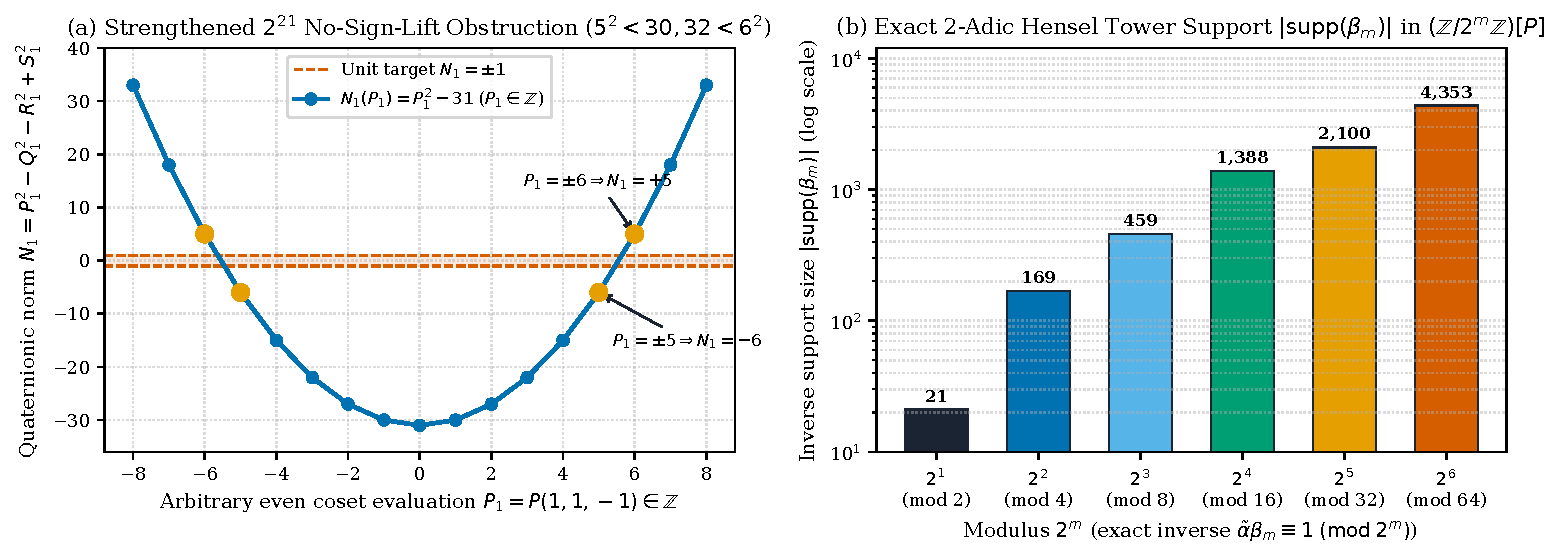
\includegraphics[width=\textwidth]{figures/fig2_gardam_sign_lift_obstruction.pdf}
  \caption{Pillar~I algebraic landscape. \textbf{(a)} Strengthened $2^{21}$ no-sign-lift
  obstruction parabola $N_1(P_1) = P_1^2 - 31$ at the quaternionic sign point $s_1 = (1,1,-1)$,
  missing the unit target $N_1 = \pm 1$ between $5^2 = 25$ and $6^2 = 36$.
  \textbf{(b)} Exponential support growth of the exact $2$-adic Hensel inverses of $\widetilde{\alpha}$
  in $(\Z/2^m\Z)[P]$ for $m = 1, \dots, 6$.}
  \label{fig:gardam}
\end{figure}

\begin{theorem}[Surjunctive Reversible $21$-Neighbor Linear CA on $\F_2^P$; \textsf{T1g}]
\label{thm:t1g}
For any commutative ring $R$ and $u \in R[P]$, the finite-range convolution map
$(\Phi_u \mathrm{cfg})(g) = \sum_{(h,c) \in u} c \cdot \mathrm{cfg}(gh)$ is strictly left
$P$-equivariant and satisfies $\Phi_u \circ \Phi_v = \Phi_{uv}$. Instantiating $(u,v) = (\alpha, \beta)$
over $\F_2[P]$ yields an explicit $21$-neighbor non-Abelian linear cellular automaton $\Phi_\alpha : \F_2^P \to \F_2^P$
that is bijective (hence injective and surjective, witnessing Gottschalk surjunctivity on $P$) with
exact $21$-neighbor finite-range inverse $\Phi_\beta$.
\end{theorem}

\section{Pillar II: All-Prime Type-II Fracton Codes and Non-Abelian Hantzsche--Wendt Stabilizers}
\label{sec:pillar2}

\subsection{Classification of All $64$ Signed Haah Cubic Codes}

Consider the $64$-member family of signed Haah cubic stabilizer codes over $\F_p[x^{\pm 1}, y^{\pm 1}, z^{\pm 1}]$
generated by
\[
  f_{\mathbf{a}} = 1 + a_1 x + a_2 y + a_3 z, \qquad
  g_{\mathbf{b}} = 1 + b_1 xy + b_2 yz + b_3 zx, \qquad
  a_i, b_i \in \{+1, -1\}.
\]
Eliminating $z = -a_3(1 + a_1 x + a_2 y)$ from $g_{\mathbf{b}} = 0$ projects the characteristic
variety $V(f_{\mathbf{a}}, g_{\mathbf{b}})$ onto a plane conic $A x^2 + B xy + C y^2 + D x + E y + F = 0$
whose symmetric $3\times 3$ matrix $2Q$ has integer determinant $\det(2Q) \in \Z$.

\begin{theorem}[Complete $64$-Signed Haah Discriminant Classification; \textsf{T2b}]
\label{thm:t2b}
Across all $64$ sign vectors $(\mathbf{a}, \mathbf{b}) \in \{\pm 1\}^6$:
\begin{enumerate}[leftmargin=2em]
  \item The projective conic discriminant $\det(2Q)$ takes six nonzero values,
    $\{-12, -8, -4, +4, +8, +12\}$, with exact multiplicities $(12, 16, 4, 4, 16, 12)$,
    partitioning all $64$ codes into four sign-gauge equivalence classes $m \in \{0,1,2,3\}$.
  \item For \emph{every} prime $p \ge 5$, $\det(2Q) \not\equiv 0 \pmod{p}$ across all $64$ codes,
    so every projected conic is geometrically smooth over $\overline{\F}_p$.
  \item At $p = 3$, exactly $24$ codes ($m=1$, $\det(2Q) = \pm 12$) degenerate into an
    $\F_9$-conjugate pair of lines meeting at an off-torus axis point---for example,
    $(1,1,1,1,1,-1)$ reduces mod~$3$ to $(x-1)^2 + (x-1)y - y^2 \equiv 0$, singular at $(1,0,1)$,
    driving a characteristic-$3$ degeneracy surge to $k_3(8) = 24$ (Figure~\ref{fig:haah}(b)).
  \item At $p = 2$, all $64$ codes collapse to Haah's original Cubic Code~1~\cite{haah2011local},
    which factors over $\F_4 = \F_2[\omega]$ as $(x + \omega y + \omega^2)(x + \omega^2 y + \omega) = 0$.
\end{enumerate}
\end{theorem}

\subsection{Universal All-Prime Type-II No-Strings Theorem and Odd-Prime Torsion}

Haah's original proof that Cubic Code~1 ($\mathbf{a}=\mathbf{b}=(1,1,1)$) admits no string logical
operators relied on characteristic-$2$ factorization over $\F_4$~\cite{haah2011local,haah2013commuting}.
We now give an elementary, purely polynomial proof valid simultaneously in \emph{every} prime
characteristic $p \ge 2$ and in characteristic~$0$.

\begin{theorem}[Universal All-Prime Type-II No-Strings Theorem; \textsf{T2c}]
\label{thm:t2c}
Define four quadratic polynomials over $\Z[t]$:
\[
  D(t) = 1 + t + t^2, \quad
  P_x(t) = -1 - 3t - t^2, \quad
  P_y(t) = 1 + t - t^2, \quad
  P_z(t) = -1 + t + t^2.
\]
Then $(x, y, z) = (P_x/D, P_y/D, P_z/D)$ rationally parametrizes the Haah CC1 curve
$V(f,g)$ ($D + P_x + P_y + P_z = 0$ and $D^2 + P_x P_y + P_y P_z + P_z P_x = 0$), and all
$\binom{4}{2} = 6$ pairs satisfy exact linear B\'ezout identities in $\Z[t]$ with right-hand side~$2$:
\begin{align*}
  (3+t)D + (1+t)P_x &= 2, & (2-t)D - t P_y &= 2, & D - P_z &= 2, \\
  (3-2t)P_x + (5+2t)P_y &= 2, & -t P_x - (2+t)P_z &= 2, & (1+t)P_y + (t-1)P_z &= 2.
\end{align*}
Consequently:
\begin{enumerate}[leftmargin=2em]
  \item Over \emph{every} integral domain $K$ with $2 \neq 0$ containing roots of $P_x, P_y, P_z$
    (in particular over $\overline{\F}_p$ for every odd prime $p \ge 3$ and over $\C$), the zero
    sets of $D, P_x, P_y, P_z$ are pairwise disjoint, so no nontrivial Laurent monomial
    $x^a y^b z^c$ ($(a,b,c) \neq (0,0,0)$) can be a nonzero constant $\lambda$ along $V(f,g)$.
  \item At $p = 2$, evaluating along the $\F_4$-line $(x(t),y(t),z(t)) = (\omega t + \omega^2, t, \omega^2 t + \omega)$
    at $t \in \{\omega, 0, \omega^2\}$ similarly forces $a = b = c = 0$.
\end{enumerate}
Hence Haah's Cubic Code~1 is strictly Type-II (string-free) in every prime qudit dimension $p \ge 2$.
\end{theorem}

\begin{theorem}[Odd-Prime Torsion Floor and First Odd-$L$ Threshold at $p=23$; \textsf{T2d}]
\label{thm:t2d}
For Haah's Cubic Code~1 over $\F_p$ with odd prime $p \ge 3$:
\begin{enumerate}[leftmargin=2em]
  \item $(1,1,1)$ is never a root ($4 \not\equiv 0 \pmod{p}$), whereas the three involution points
    $(-1,1,-1)$, $(1,-1,-1)$, $(-1,-1,1)$ always lie on $V_p(f,g)$, yielding a universal even-torus
    degeneracy floor $k_p(L) \ge 6$ for every even $L$, punctuated by Frobenius $6p$ jumps at $L = 2p$
    (e.g., $k_3(6)=18$, $k_5(10)=30$, $k_7(14)=42$; Figure~\ref{fig:haah}(a)).
  \item For all odd primes $p \in \{3, 5, 7, 11, 13, 17, 19\}$, $V_p(f,g)$ contains \emph{zero}
    $\F_p$-rational odd-order torsion points.
  \item The first odd prime admitting an $\F_p$-rational odd-order root is $p = 23$ at odd linear
    size $L = 11$, yielding $k_{23}(11) = 6$, followed by $p = 31$ at $L = 15$.
\end{enumerate}
\end{theorem}

\begin{figure}[htbp]
  \centering
  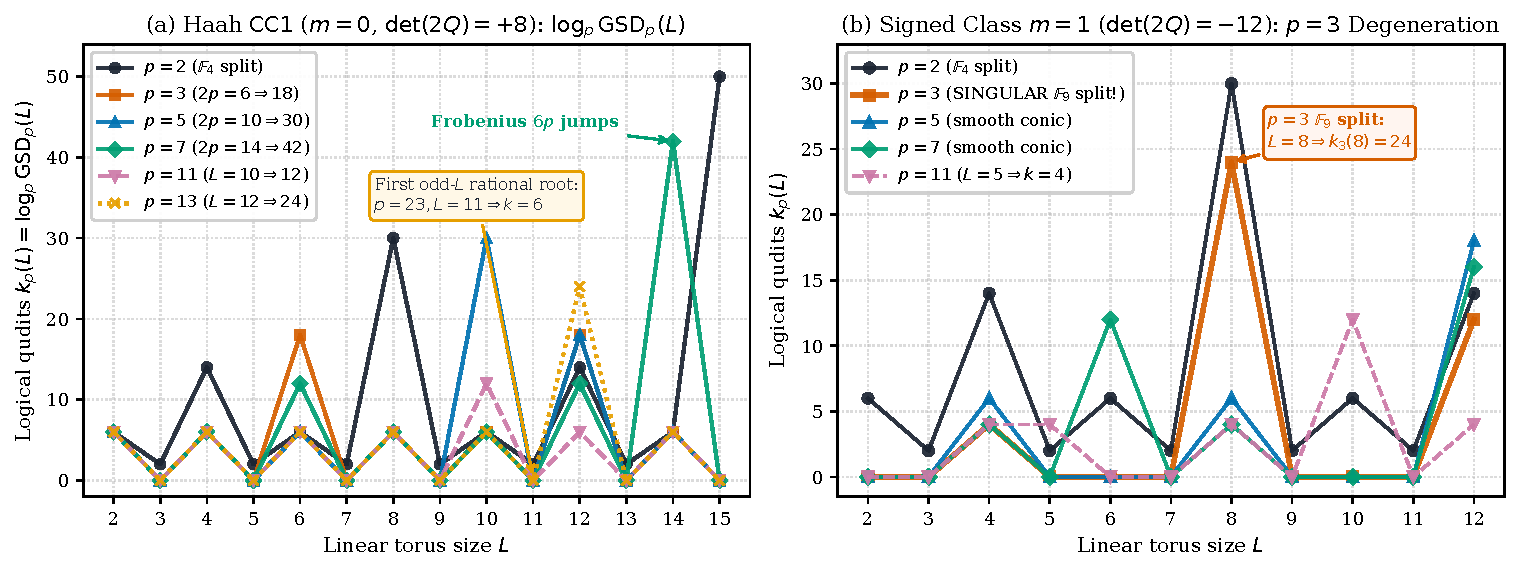
\includegraphics[width=\textwidth]{figures/fig1_haah_prime_bifurcation.pdf}
  \caption{Pillar~II arithmetic fracton spectrum. \textbf{(a)} Exact logical qudit count
  $k_p(L) = \log_p \GSD_p(L)$ for Haah $\mathrm{CC1}$ across primes $p \in \{2,3,5,7,11,13\}$,
  highlighting Frobenius $6p$ jumps at $L=2p$ and the first odd-$L$ rational root threshold at
  $p=23, L=11$ ($k_{23}(11)=6$). \textbf{(b)} Signed class $m=1$ ($\det(2Q)=-12$), illustrating
  the $p=3$ singular $\F_9$ degeneration driving $k_3(8)=24$.}
  \label{fig:haah}
\end{figure}

\subsection{First Non-Abelian Hantzsche--Wendt Fracton Stabilizer Codes}

\begin{theorem}[Unit-Twisted and Intrinsically Non-Abelian HW Fracton Codes; \textsf{T2a}, \textsf{T2e}]
\label{thm:t2ae}
\leavevmode
\begin{enumerate}[leftmargin=2em]
  \item Over any associative involutive ring $R$ satisfying $(xy)^* = y^* x^*$ and $x^{**} = x$,
    if $fg = gf$ and $uv = 1$, then the non-Abelian CSS checks $H_X = (fu,\, gu)$ and
    $H_Z = (g^* v^*,\, -f^* v^*)$ obey exact symplectic commutation $H_X H_Z^\dagger = 0$.
  \item \emph{(Gardam-Twisted Haah Code on $P$.)} Choosing $(f,g)$ as Haah's CC1 generators in
    $R[N] \subset R[P]$ and $(u,v) = (\alpha, \beta)$ gives a non-Abelian stabilizer code on the
    Hantzsche--Wendt $3$-manifold with exact check weights $(52, 52)$ ($H_X$) and $(52, 56)$
    ($H_Z$) that commutes strictly in $\F_2[P]$ (preserving $k(M_L) = 4 k_{\mathrm{Haah}}(L)$ on
    $L$-folded covers) while \emph{failing} to commute over $\Z[P]$, where the exact integer
    commutator defect has $342$ nonzero even terms. Its CSS commutativity is thus an algebraic
    consequence of Gardam's counterexample to Kaplansky's Unit Conjecture.
  \item \emph{(Intrinsically Non-Abelian Ring-Universal HW Code.)} The pair
    $f_{\mathrm{HW}} = 1 + a + b + ab$ and $g_{\mathrm{HW}} = 1 + x + x^{-1} + y + y^{-1} + z + z^{-1}$
    commutes identically over $\Z[P]$---hence over \emph{every} commutative ring $R[P]$---while
    $f_{\mathrm{HW}}$ is strictly non-central ($f_{\mathrm{HW}} x \neq x f_{\mathrm{HW}}$).
\end{enumerate}
\end{theorem}

\section{Pillar III: 3D Non-Hermitian Amoebae, $V_4$-Convex Ronkin Minima, and Full $S_4$ Monodromy}
\label{sec:pillar3}

In the amoeba formulation of multi-dimensional non-Bloch band theory~\cite{passare2004amoebas,wang2024amoeba},
a $3$D non-Hermitian Bloch Hamiltonian $H(k)$ with characteristic polynomial $P_E(e^{ik}) = \det(H(k) - E I)$
has amoeba $\A(P_E) = \{ \mu \in \R^3 : \exists k \in \T^3,\; P_E(e^{\mu + ik}) = 0 \}$ and convex
Ronkin potential
\[
  R_E(\mu) = \int_{\T^3} \frac{d^3k}{(2\pi)^3} \log \bigl| P_E(e^{\mu + ik}) \bigr|.
\]
The gradient $\nabla_\mu R_E(\mu)$ vanishes at the open-boundary-condition (OBC) skin decay rate
$\mu_{\min}$; a nonzero $\mu_{\min}$ signifies directional non-Hermitian skin localization.

\begin{theorem}[$V_4$-Convex Ronkin Minimum and Haah Double-Amoeba; \textsf{T3a}, \textsf{T3b}]
\label{thm:t3ab}
\leavevmode
\begin{enumerate}[leftmargin=2em]
  \item Let $R : \Q^3 \to \Q$ be midpoint-convex and invariant under the three $V_4$ sign reflections
    $(\mu_x,-\mu_y,-\mu_z)$, $(-\mu_x,\mu_y,-\mu_z)$, and $(-\mu_x,-\mu_y,\mu_z)$ (a symmetry forced
    on every Hantzsche--Wendt Bloch operator $\Psi(u)$ by Theorem~\ref{thm:t1cd}(1)). Then $R$
    attains its global minimum at the origin:
    \[
      \forall \mu \in \Q^3, \qquad R(0,0,0) \le R(\mu).
    \]
    Consequently, the $x$-axis spectral winding obeys exact bipolar antisymmetry,
    $W_x(k_y, -k_z) = -W_x(k_y, k_z)$, across every gapped slice of $\T^2$.
  \item In radius coordinates $(r_x, r_y, r_z) = (e^{\mu_x}, e^{\mu_y}, e^{\mu_z}) > 0$, the Haah
    double-amoeba $\A(f) \cap \A(g)$ is governed by exact quadrilateral triangle inequalities
    ($1 \le r_x + r_y + r_z$, $r_x \le 1 + r_y + r_z$, etc., and their quadratic counterparts),
    contains the entire positive diagonal $(r,r,r)$ for $r \ge 1$ (including the origin $\mu = 0$),
    and exits $\A(f)$ along $(r,1,1)$ for all $r \ge 4$. At any single-generator root ($f=0, g \neq 0$),
    the off-diagonal Haah Dirac operator $H = \begin{psmallmatrix} 0 & f \\ g & 0 \end{psmallmatrix}$
    over any integral domain is an algebraic second-order exceptional point ($\mathrm{EP}_2$):
    $H \neq 0$, $H^2 = 0$, and every null vector $(v_0, v_1)$ satisfies $v_0 = 0$.
\end{enumerate}
\end{theorem}

\begin{figure}[htbp]
  \centering
  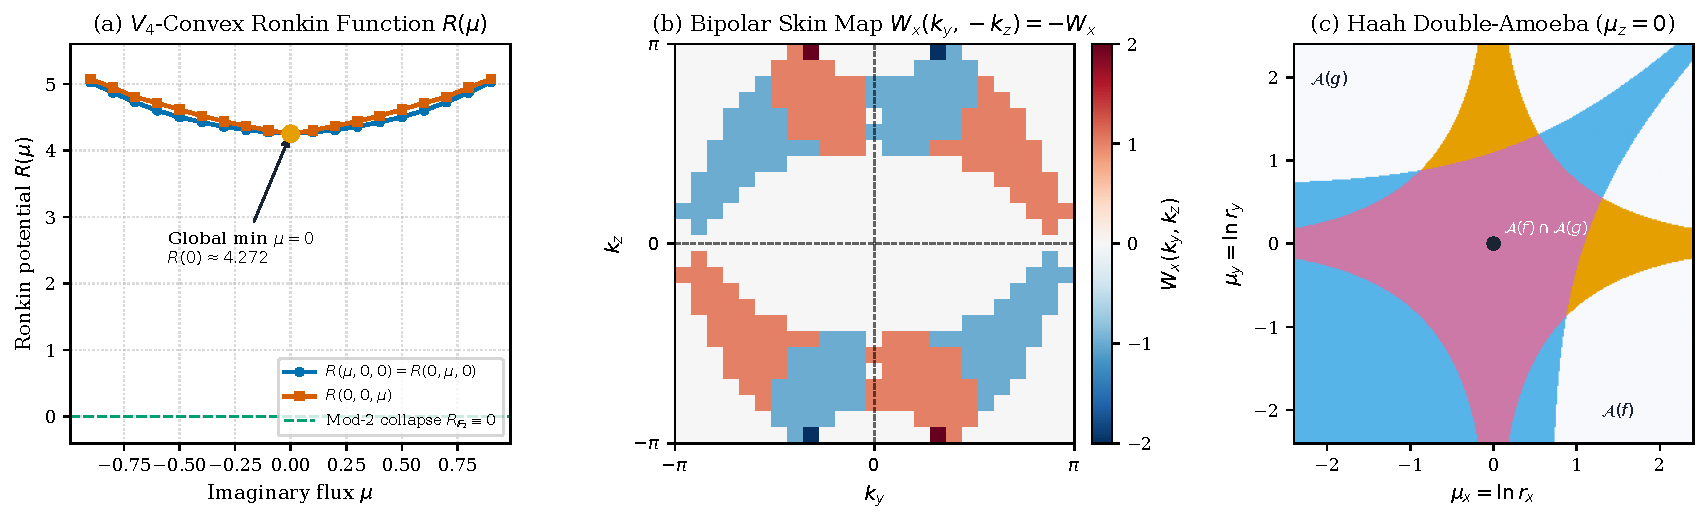
\includegraphics[width=\textwidth]{figures/fig3_nonhermitian_amoeba_ronkin.pdf}
  \caption{Pillar~III non-Hermitian amoeba and bipolar skin geometry (\tierN{}).
  \textbf{(a)} $V_4$-convex Ronkin potential $R(\mu)$ of Gardam's $4$-band Bloch crystal
  $\Psi(\widetilde{\alpha})$, attaining its global minimum at $\mu = 0$ ($R(0) \approx 4.272$,
  versus exact mod-$2$ collapse $R_{\F_2} \equiv 0$).
  \textbf{(b)} Spectral winding map $W_x(k_y,k_z)$ on a $25 \times 25$ gapped grid showing exact
  bipolar antisymmetry $W_x(k_y,-k_z) = -W_x(k_y,k_z)$ ($\max|\mathrm{err}| = 0.0$, nonzero
  fraction $42.6\%$).
  \textbf{(c)} Slice $\mu_z = 0$ of Haah's double-amoeba $\A(f)\cap\A(g)$ containing $\mu = (0,0,0)$.}
  \label{fig:amoeba}
\end{figure}

\subsection{Full Non-Abelian $S_4$ Eigenvalue Monodromy of Gardam's Crystal}

Along any gapped $1$D cycle $\gamma \subset \T^3$, the $4$ distinct complex eigenvalues
$\{\lambda_0(t),\dots,\lambda_3(t)\}$ of $\Psi(\widetilde{\alpha})(k(t))$ trace a closed $4$-strand
braid in Artin's braid group $B_4$~\cite{wojcik2020homotopy,hu2021knots}. Rather than relying on a
projection-dependent crossing count, we measure the coordinate-free \emph{canonical quartic
discriminant braid degree}
\[
  \deg_\Delta(\gamma) = \frac{1}{2\pi} \oint_\gamma d\arg \Disc\bigl(\det(\lambda I_4 - \Psi(\widetilde{\alpha})(k))\bigr) \in \Z.
\]

\begin{theorem}[Artin $B_4$ Relations and Full $S_4$ Monodromy Generation; \textsf{T3c}]
\label{thm:t3c}
The adjacent-band generators $\sigma_1, \sigma_2, \sigma_3$ satisfy the Artin $B_4$ relations
$\sigma_1\sigma_2\sigma_1 = \sigma_2\sigma_1\sigma_2$, $\sigma_2\sigma_3\sigma_2 = \sigma_3\sigma_2\sigma_3$,
and $\sigma_1\sigma_3 = \sigma_3\sigma_1$. Moreover, the exact permutations realized by Gardam's
$4$-band Bloch crystal $\Psi(\widetilde{\alpha})(k)$ along gapped fundamental cycles of $\T^3$
(Table~\ref{tab:braids}, Figure~\ref{fig:braids})---specifically the transposition $g_{x1} = (1\,2)$
and the $4$-cycle $g_{x2} = (0\,2\,1\,3)$---do not commute and generate the \emph{entire}
non-Abelian symmetric group $S_4$ of order~$24$.
\end{theorem}

\begin{table}[htbp]
\centering
\caption{Canonical quartic discriminant braid degrees and band permutations for $\Psi(\widetilde{\alpha})(k)$ (\tierN{} with verified eigenvalue gap bounds; $S_4$ closure \tierK{}).}
\label{tab:braids}
\footnotesize
\setlength{\tabcolsep}{5pt}
\begin{tabular}{@{}lcccc@{}}
\toprule
\textbf{Momentum Cycle $\gamma \subset \T^3$} & \textbf{Min Gap} & \textbf{Permutation $\pi_\gamma$} & \textbf{Cycle Type} & \textbf{$\deg_\Delta(\gamma)$} \\
\midrule
$k_x \in [0,2\pi],\; (k_y,k_z) = (0.3, 0.7)$ & $0.4841$ & $[0,2,1,3]$ & $(1\,2)$ & $-1$ \\
$k_x \in [0,2\pi],\; (k_y,k_z) = (1.0, 1.5)$ & $1.5925$ & $[2,3,1,0]$ & $(0\,2\,1\,3)$ & $-3$ \\
$k_z \in [0,2\pi],\; (k_x,k_y) = (2.0, 1.0)$ & $1.4901$ & $[1,0,3,2]$ & $(0\,1)(2\,3)$ & $-2$ \\
$k_y \in [0,2\pi],\; (k_x,k_z) = (1.0, 1.5)$ & $2.1502$ & $[3,2,0,1]$ & $(0\,3\,1\,2)$ & $+3$ \\
\bottomrule
\end{tabular}
\end{table}

\begin{figure}[htbp]
  \centering
  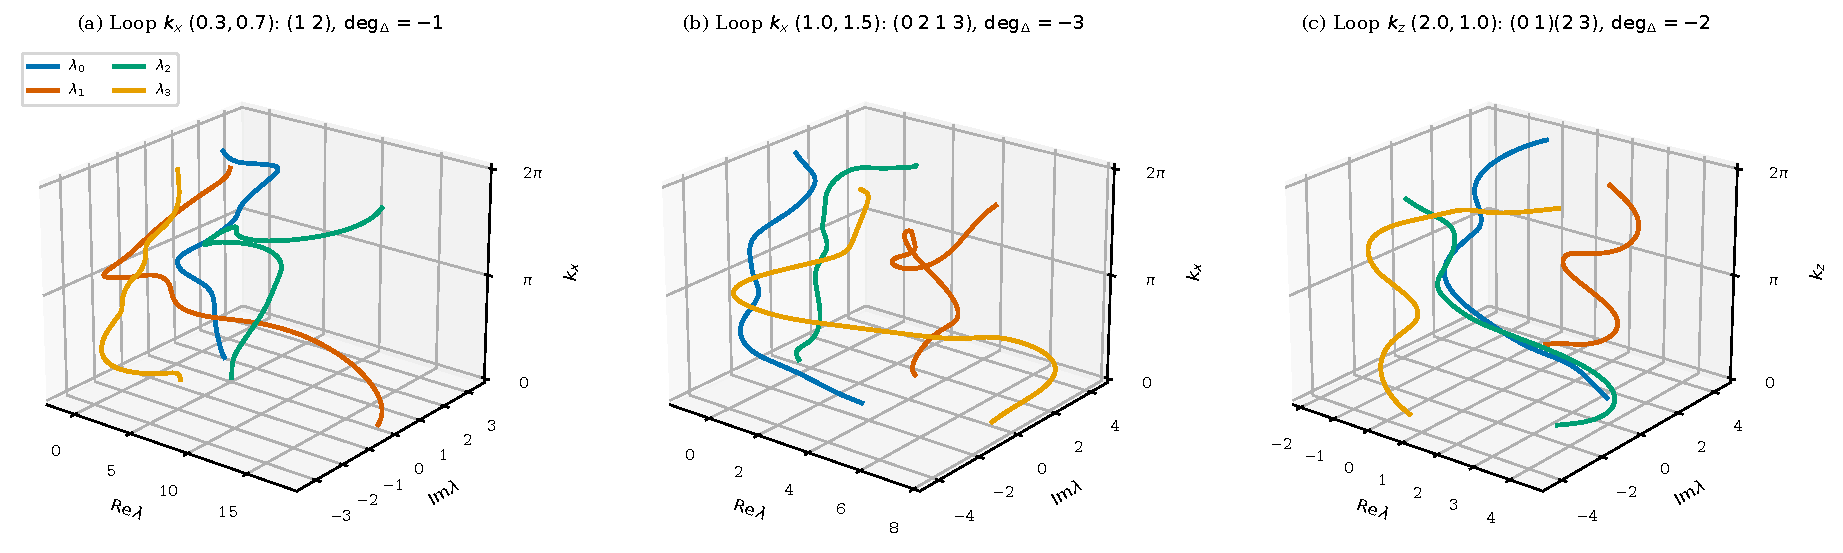
\includegraphics[width=\textwidth]{figures/fig4_b4_eigenvalue_braids.pdf}
  \caption{Three-dimensional non-Hermitian $B_4$ eigenvalue braids of Gardam's $4$-band
  Hantzsche--Wendt crystal $\Psi(\widetilde{\alpha})(k)$ around fundamental $\T^3$ loops realizing
  \textbf{(a)} transposition $(1\,2)$ ($\deg_\Delta=-1$), \textbf{(b)} $4$-cycle $(0\,2\,1\,3)$
  ($\deg_\Delta=-3$), and \textbf{(c)} double transposition $(0\,1)(2\,3)$ ($\deg_\Delta=-2$).
  Together, (a) and (b) generate the full non-Abelian symmetric group $S_4$ of order~$24$.}
  \label{fig:braids}
\end{figure}

\section{Formal Verification Architecture, Statement Fidelity, and Limitations}
\label{sec:verification}

\subsection{Zero-Mathlib Six-Kernel Trust Base}

Every theorem in Table~\ref{tab:claims} marked \tierK{} is formalized from first principles in
Lean~4.35.0 (\texttt{lean/}) using the \texttt{module} header discipline and \emph{zero} Mathlib imports.
To eliminate specification-cheating and single-kernel risk, the Lean suite enforces four
independent safeguards:
\begin{enumerate}[leftmargin=2em]
  \item \textbf{Axiom purity:} \texttt{VerifyAxioms.lean} audits \texttt{\#print axioms} for every
    headline theorem and master conjunction, confirming zero \texttt{sorryAx}, zero
    \texttt{native\_decide} or \texttt{Lean.ofReduceBool}, and zero custom axioms---strictly within
    $\{\texttt{propext}, \texttt{Classical.choice}, \texttt{Quot.sound}\}$.
  \item \textbf{Palomar Challenge/Solution separation:} \texttt{PalomarChallenge.lean} fixes the
    untrusted public theorem signatures independently of \texttt{PalomarSolution.lean}, checked
    under \texttt{lake comparator --paranoid} using \texttt{comparator.json}.
  \item \textbf{Six independent proof kernels:} Continuous integration replays the proof terms
    through (i)~the default Lean~4.35.0 kernel, (ii)~\texttt{leanchecker-paranoid},
    (iii)~\texttt{lean4lean}, (iv)~\texttt{nanoda\_bin}, (v)~\texttt{con-leche --verified}, and
    (vi)~\texttt{con-ron --verified}.
  \item \textbf{Non-vacuity and adversarial refutations:} \texttt{NonVacuity.lean} inhabits every
    custom typeclass hypothesis (including an integral-domain instance on \texttt{ZMod 11},
    concrete roots of $P_x, P_y, P_z$, a convex $V_4$-symmetric rational Ronkin function, and
    explicit primes $5, 23$), while \texttt{AdversarialTests.lean} constructively refutes five
    deliberate false variants inside the kernel.
\end{enumerate}

\subsection{Limitations and Threats to Validity}

\begin{itemize}[leftmargin=2em]
  \item \textbf{Characteristic-zero Unit Conjecture remains open:} Theorem~\ref{thm:t1ef}(2) rules
    out all $2^{21}$ sign lifts of Gardam's $21$-element support (and arbitrary even-sum
    $p \in \Z[N]$ paired with Gardam's $(q,r,s)$ supports), but does \emph{not} rule out larger
    supports or non-$\{\pm 1\}$ integer coefficients in $\Z[P]^\times$ or $\Q[P]^\times$.
  \item \textbf{Numerical approximations are explicitly separated:} The Ronkin quadrature values
    ($R(0) \approx 4.271743$ on an $N=16$ $3$D grid, converging at $O(1/N)$ across $1$D logarithmic
    nodal curves where $\det\Psi = 0$), the $25 \times 25$ winding map (using a gap filter
    $\min|\det| > 0.35$), and the $600$-step complex eigenvalue tracks ($1024$-step for
    $\deg_\Delta$) are floating-point computations (\tierN{}). While differentially verified between independent Rust and Python
    implementations to $< 10^{-6}$ and accompanied by positive spectral gap bounds, they are not
    certified by interval arithmetic inside Lean.
  \item \textbf{Exact $2$-adic tower vs.\ $2$-adic convergence:} The Hensel tower proves
    invertibility in $(\Z/2^m\Z)[P]$ for every finite $m \ge 1$; its inverse supports grow rapidly
    ($21 \to 4353$ by $m=6$), giving an inverse in the completed ring $\Z_2[[P]]$, not a finitely
    supported unit in $\Z[P]$.
  \item \textbf{Finite-size code distance:} Theorem~\ref{thm:t2ae}(2)--(3) proves exact non-Abelian
    CSS commutation and stabilizer weights; deriving asymptotic code-distance scaling laws for
    non-Abelian Hantzsche--Wendt covers $M_L$ remains an open research direction.
\end{itemize}

\section{Reproducibility, AI-Assistance Disclosure, and Data Availability}
\label{sec:repro}

\textbf{Reproducibility.} All formal proofs, Rust and Python verifiers, test suites (including
Hypothesis property tests, Rust$\leftrightarrow$Python differential checks, and semantic mutation
testing), vector figures, and the real-time $3$D WebGL2 interactive studio + Lean proof blueprint
are archived openly at \url{https://github.com/0thernes/promislow-fracton-amoeba} (tag \texttt{v1.0.0})
with pinned toolchains (\texttt{leanprover/lean4:v4.35.0}, Rust~1.94, Python~3.13, Tectonic~0.17.0)
and SHA-256 manifests (\texttt{MANIFEST.sha256}). See \texttt{REPLICATION.md} for exact clean-clone
commands.

\textbf{AI-Assistance Disclosure and CRediT Roles.} Alexander Stephen Donahue conceived the
research program, selected the Hantzsche--Wendt / fracton / amoeba synthesis, directed all
mathematical conjectures and adversarial audits, reviewed every theorem boundary and limitation,
and bears sole scholarly responsibility for the paper. AI assistance (Google Antigravity / Gemini)
was used under continuous human direction for zero-Mathlib Lean~4.35.0 proof engineering, Rust and
Python verification implementation, interactive WebGL2 visualization, figure generation, and
manuscript drafting. Every formal claim was independently verified by six proof kernels and every
cited bibliographic reference was checked live against Crossref and arXiv APIs.

\textbf{Competing Interests.} The author declares no competing financial or non-financial interests.

\textbf{License.} Code and formal proofs are licensed under Apache-2.0; manuscript prose, figures,
and verification reports are licensed under CC-BY-4.0.

\bibliographystyle{amsplain}
\bibliography{references}

\end{document}
